\documentclass{article} %[twocolumn] 

%\usepackage{algorithmic}
\usepackage{algorithm}
\usepackage{algorithmicx}
\usepackage{algpseudocode}
\usepackage{booktabs}
\usepackage{array}
\usepackage{graphicx}
\usepackage{amsmath}
\usepackage{amsfonts}
\usepackage{amssymb}
\usepackage{multirow}

\title{Efficient and flexible simulation-based design of complex clinical trials}
\date{}

\begin{document}

\maketitle

\begin{abstract}
\textbf{Background}: Simulation provides a flexible means with which to estimate clinical trial operating characteristics, allowing complex trial design problems to be addressed without the need for simplifying, yet unrealistic, assumptions. The computational burden of using simulation has, however, restricted its application to only the simplest of trial design problems. These typically involve minimising a single parameter (the sample size) subject to constrained operating characteristics. Many problems of optimal trial design are more complex, requiring optimisation over several parameters to minimise several criteria, subject to several constraints. For the benefits of simulation-based design to be fully realised, a general framework for optimal trial design in problems of this sort is required. In this paper we define such a framework and show how efficient optimisation algorithms can be used to solve these problems in an effective, timely manner.

\textbf{Methods}: We describe a general framework for solving multi-objective trial design problems using Bayesian optimisation. Given estimated operating characteristics of a set of designs generated using simulation, a non-parametric regression model is fitted and used to predict operating characteristics of new designs. These predictions, and their associated uncertainty, are used at each iteration to carefully select the design to be evaluated next. The method is flexible, can be used for almost any problem for which operating characteristics can be estimated using simulation, and can be implemented using existing statistical software packages.

\textbf{Evaluation}: The framework is illustrated using two examples of complex trial design: a cross-classified psychotherapy trial, and a cluster-randomised pilot trial with co-primary endpoints. Simulation studies comparing the proposed approach to a simpler alternative demonstrate the efficiency of the proposed approach.

\textbf{Conclusions}: Bayesian optimisation can be an effective method for complex trial design problems where operating characteristics must be estimated using simulation. By improving the efficiency of these calculations, increasingly complex trial design problems can be addressed without the need for unrealistic assumptions.
\end{abstract}

\section{Introduction}\label{sec:intro}

%\cite{Reich2012} - Empirical Power and Sample Size Calculations for Cluster-Randomized and Cluster-Randomized Crossover Studies
%Proposes to use simulation for estimating power in cluster-randomised crossover studies. Doesn't explicitly consider methodology for SSD using these estimates, and in the examples only considers problems with a single design variables. Simulation function is in R, not C++ - and uses a for loop! Not much use.

%\cite{Sutton2007} - Evidence-based sample size calculations based upon updated meta-analysis. Simulation approach, ``Although for simple situations closed form solutions are often possible,for more complex analyses, including those that include random effects, closed form solutionsoften do not exist and simulation methods become an appealing alternative''. Refers to~\cite{Feiveson2002} for a general guide. Later argues that even if closed form solutions could be derived, the flexibility of the simulation approach is preferable.

%When designing a clinical trial to test a hypothesis it is typical to choose the smallest sample size which will ensure the power of the trial is above some nominal threshold. When analytical formulae for calculating power are available, the computations required to determine this sample size can be carried out quickly. However, such power formulae are not always available. An alternative is to compute Monte Carlo (MC) estimates of power~\cite{Landau2013}. An MC estimate can be obtained by simulating trial data under the alternative hypothesis many times, analysing each data set, and calculating the proportion of times the null hypothesis is rejected. Although the estimate includes some error, it is unbiased and the magnitude of the error can be reduced to the desired amount by increasing the number of the samples which form the estimate is formed~\cite{Robert2004}. The method is both conceptually simple and highly flexible, being applicable to almost any model of data generation and analysis. These qualities have led to simulation-based power calculation and sample size determination being advocated in applied and medical research~\cite{Arnold2011, Landau2013} and used in a broad range of settings. Examples include designs involving hierarchical models~\cite{Wang2002, Hooper2013}, proportional hazards models~\cite{Schoenfeld2005}, logistic regression models~\cite{Grieve2016}, individual patient data meta-analyses~\cite{Kontopantelis2016}, stepped wedge designs~\cite{Baio2015, Hooper2016} and adaptive designs~\cite{Wason2012}.

%Include \cite{Fedorov2005} - The design of multicentre trials. In Section 12 they use simulation to assess designs, allowing them to model recruitment processes and randomisation methods - ``We have given simple formulae which show, in ideal settings, what the effect will be of random enrolment and various degrees of the within-centre and between-centre variation. Results for more realistic scenarios can be obtained via simulation.''

%\cite{Feng1992} - Correlated binomial variates: Properties of estimator of intraclass correlation and its effect on sample size calculation

% MC power calcs are simple, flexible, widely used / advocated
The optimal design of a clinical trial is typically framed as a constrained optimisation problem, where we choose the design with smallest sample size such that power is above some nominal bound. When a simple analytical expression for power is not available, a Monte Carlo (MC) estimate can be used instead~\cite{Arnold2011, Landau2013}. This can be obtained by simulating trial data under the alternative hypothesis many times, analysing each data set, and calculating the proportion of times the null hypothesis is rejected. The method is both conceptually simple and highly flexible, being applicable to any trial design where the data generating process and the analysis can be simulated. It has been used in a numerous settings, including problems involving hierarchical models~\cite{Feng1992, Hooper2013}, proportional hazards models~\cite{Schoenfeld2005}, logistic regression models~\cite{Grieve2016}, individual patient data meta-analyses~\cite{Sutton2007, Kontopantelis2016}, patient enrolment models~\cite{Fedorov2005}, stepped wedge designs~\cite{Baio2015, Hooper2016}, and cluster randomised crossover designs~\cite{Reich2012}. 

% MC calcs are computationaly demanding for SSD
The flexibility afforded by the simulation approach comes at the cost of computation time. Nonetheless, the optimal design for a clinical trial can be found reasonably quickly in simple cases. For example, consider a trial design problem where we must choose the per-arm sample size $n$ from within some feasible range $[0,  n_{m}]$. We aim to find the smallest $n$ such that the trial will be powered at the nominal level, say 80\%. A simple bisection search can be used to find this optimal $n$ and will require no more than 
$\lfloor \log_{2}{n_{m}}+1 \rfloor$ iterations. If the upper limit on the sample size was $n_{m} = 800$, for example, at most 10 simulations will be required. Thus, even if computing an MC estimate of power takes several minutes, the optimal design problem can still be solved in a timely manner. A general framework for simulation-based trial design in problems of this nature is given in~\cite{Landau2013}.

% Scope of the paper - problems which are hard to do SSD via MC
In this paper we focus on trial design problems which are more complicated, in at least two respects. Firstly, we consider problems with several \emph{design parameters} which influence operating characteristics and are determined as part of the trial design. For example, in cluster randomised trials both the number of clusters, and the number of participants in each cluster, must be chosen. As the number of design parameters increases, so too does the set of possible designs which must be searched over, and the computational burden of MC power calculations begins to have stronger implications. Secondly, we consider problems where we wish to obtain not a single optimal design, but a range of designs which lead to the desired operating characteristics and offer different balances between multiple criteria we wish to minimise. The aforementioned cluster randomised design also exhibits this feature, as we aim to minimise both the number of clusters and the total number of participants, recognising that these objectives will be in conflict. Seeking to find a set of good designs rather than a single optimum further adds to the difficulty of the problem.

%A framework for using simulation to estimate power and choose sample size is given in~\cite{Landau2013}. However, it is applied only to sample size determination (SSD) problems with a single design variable, such as the number of participants in each arm of a balanced RCT. Each of the aforementioned examples of simulation-based SSD were also of this nature. Many SSD problems are more complicated and involve choosing the values of several design parameters. For example, consider the design of a cluster randomised trial where both the number of clusters and the number of participants in each cluster must be chosen. As the number of design variables increases, the number of potential trial designs which must be considered increases, and so the computational burden incurred when using simulation to estimate power is more keenly felt. In particular, SSD problems in more than one variable cannot be solved using simple algorithms such as a bisection search.

%The sample size is often defined by a single design parameter $n$. Sample size determination (SSD) problems of this nature are particularly straightforward to solve. For example, given a maximum value of $n$ which would be considered feasible, a simple bisection search could be used to find the lowest $n$ such that the power of the resulting trial will be above the nominal threshold. Other SSD problems are complicated by the presence of multiple design parameters. For example, in some cluster randomised trials we may be required to choose both the number of clusters and the number of participants in each cluster. 

%The benefits of the simulation method come at the cost of computation time. A typical recommendation is that thousands of samples should be generated in order to obtain a sufficiently precise estimate~\cite{Landau2013, Baio2015} (although a broad range of alternatives, from $N = 100$~\cite{Landau2013} to $N = 250,000$~\cite{Wason2012}, have been used). When the generation of each sample involves a computationally demanding procedure such as fitting a multilevel model, it can take several minutes to estimate the power of just one potential trial design. Nevertheless, many trial design problems are simple enough to require the evaluation of only a handful of designs before the optimum is found. In particular, problems which have only one design variable (e.g. the group size in a two-arm balanced RCT), with one quantity to be minimised (e.g. the total sample size), subject to a single constraint (e.g. power under the alternative hypothesis), can be solved using a simple bisection search. This algorithm will require no more than $\lfloor \log_{2}{n_{max}}+1 \rfloor$ iterations where $n_{max}$ is the maximum feasible value of the variable\footnote{For example, given an upper limit on the sample size of $n_{max} = 800$, at most 10 MC evaluations will be required to find the optimal sample size.}. A general framework for simulation-based trial design in problems of this nature is given in~\cite{Landau2013}.

%The benefits of the simulation method come at the cost of computation time. Simulating a sufficiently large
%\footnote{Typical recommendations for the number of simulations required to estimate power are in the range of $10^3$ to $10^5$.}
%number of data sets and carrying out the analysis on each one can often take several minutes. In simple cases, finding the sample size which provides sufficient power can nevertheless be conducted reasonably quickly. In particular, problems which have only one design variable (e.g. the group size in a two-arm balanced RCT), with one quantity to be minimised (e.g. the total sample size), subject to a single constraint (e.g. power under the alternative hypothesis), can be solved with only a handful of iterations
%\footnote{A simple bisection search algorithm will require no more than $\lfloor \log_{2}{n_{max}}+1 \rfloor$ iterations where $n_{max}$ is the maximum feasible value of the variable. For example, given an upper limit on the sample size of $n_{max} = 800$, at most 10 MC evaluations will be required to find the optimal sample size.}.
%As the complexity of the design problem grows, however, a standard optimisation algorithm will often require thousands of iterations before converging on a optimal (or near-optimal) solution. When analytic power expressions are not available and MC estimates are being used in their place, this process can take days.

%Efficiency can be improved further by employing more sophisticated algorithms such as that used in the Stata package SimSam~\cite{Hooper2013}, which limits the number of MC samples used in the early stages of the search and increases them as it converges on the optimal sample size. 

%Many trial design problems are more complicated. For example, the two-stage phase II trial design for a single binary endpoint proposed in~\cite{Simon1989} is defined by four variables: the number of patients in stage 1; the number of responses which must be observed to proceed to stage two; the number of patients in stage 2; and the total number of responses which must be observed to proceed to a phase III trial. Their optimal values are those which minimise the total sample size of the study whilst ensuring type I error and power are within nominal bounds. In contrast to a single variable problem, a multi-variable problem involves a large number of candidate designs which must be optimised over. %This optimisation is feasible in this example because type I error rate and power can be calculated quickly using exact analytic expressions. When simulation is required, standard algorithms, which can require thousands of iterations, may take days to find the optimal design.

%Often there are several distinct quantites which we wish to minimise when designing a trial. For example, in many cluster randomised trials we wish to minimise both the number of clusters and the number of patients. This problem is typically dealt with by fixing the number of patients per cluster and then minimising the number of clusters~\cite{Donner2000}, or vice-versa~\cite{Hemming2011}. Alternatively, a function which specifies the cost of sampling at the cluster and the patient level could be specified, and the overall cost minimised~\cite{Snijders1993}. The latter approach has been suggested for both two-level and three-level hierarchical trial designs~\cite{Breukelen2012, Teerenstra2008}. The \emph{a priori} specification of such a cost function may not always be feasible. An alternative approach to addressing multiple objectives is to search not for a single optimal design, but for a set of designs which offer a range of trade-offs between the objectives. Specifically, we aim to find designs which are \emph{Pareto optimal}, meaning that there is no other design which is better in at least one aspect whilst being at least as good in all others\footnote{An equivalent concept in statistical decision theory is an \emph{admissible} design.}. 
%The search for a set of designs, as opposed to a single optimum, will increase the computational cost of the design problem.
%\footnote{When fast, analytic expressions of power are available, a set of Pareto optimal designs may be found quickly using standard multi-objective optimisation algorithms such as NSGA-II~\cite{Deb2002}, as implemented in the R package mco~\cite{Mersmann2014}.}

%Finally, there may be several hypotheses at which we wish to constrain power to be within some nominal threshold, with each of these estimated using simulation. This will be the case whenever the type I error rate cannot be deduced analytically, as in the multi-stage adaptive design proposed in~\cite{Wason2011}; or when multiple outcomes lead to multiple alternative hypotheses, as in the two-stage phase II design proposed in~\cite{Sill2012}. With each rejection rate to be estimated the time needed to evaluate the properties of a single design will increase, and the design problem will become yet more computationally demanding.

% Current software / method availability
Currently, there is a lack of methodology and associated software for general simulation-based trail design. Where simulation-based methods have been proposed, they have typically focussed on a specific area of application. MLPowSim~\cite{Browne2009} makes use of the MLwiN software for multilevel analysis, and can estimate the power of a variety of multilevel trial designs at a set of evenly spaced design points. The ipdpower package in Stata was motivated by problems in individual patient data meta-analysis, although can be applied to any problem with a two-level nested structure. Sample size determination for stepped wedge trials is addressed in the R package SWSamp~\cite{Baio2015}. The Stata package SimSam~\cite{Hooper2013} is more general, allowing the user to fully specify their own data generation and analysis models. It has been applied to multilevel designs~\cite{Hooper2013}, designs for logistic regression~\cite{Grieve2016}, and stepped wedge designs~\cite{Hooper2016}. It is, however, restricted to the minimisation of a single objective, over a single variable, with the simulation of a single power constraint. 

% Proposed solution, using surrogate modelling and EGO
If we are to extend the ideas of simulation-based trial design to more complex problems, we require a more general framework employing more efficient optimisation algorithms. Outwith the context of clinical trial design a great deal of research has addressed optimisation problems where the evaluation of a solution is a computationally demanding, or \emph{expensive}, operation (see~\cite{Sacks1989} for an early review). One approach addresses the problem by substituting the expensive function with an approximation known as a \emph{surrogate model}. If the surrogate model is a good approximation of the real function and is cheap to evaluate, the time required to solve the optimisation problem can be dramatically reduced~\cite{Jones2001}.  In this paper we will explore how complex simulation-based clinical trial design problems can be solved using a particular type of surrogate model, Gaussian process regression, and associated efficient optimisation algorithms. Our focus is on flexibility, and so we will not impose any restrictions regarding the nature of the endpoint(s), underlying statistical model, test statistic, or acceptance region, other than that the data generation and analysis can be simulated.

% Structure of paper
The remainder of the paper is structured as follows. Two motivating problems are described in Section~\ref{sec:examples}. In Section~\ref{sec:prelim} we provide the necessary background and notation regarding Monte Carlo estimation and multi-objective optimisation. In Section~\ref{sec:methods} we describe Gaussian process regression, an efficient global optimisation algorithm, and a framework for their application to optimal trial design. We return to the examples in Section~\ref{sec:application}, illustrating how the framework can be applied in practice. A simulation study comparing the performance of the proposed methodology with a simpler alternative approach is reported in Section~\ref{sec:simulation}. We conclude with a discussion of the implications and limitations of the proposed approach in Section~\ref{sec:discussion}.

%Key point to emphasise - we are interested in quite general design methods which we can apply to a wide range of problems, i.e. anything we can simulate. Simulation is largely needed because the models are complex and idiosyncratic, with no literature devoted to them because this may be the first time they have come up. So for method to be useful it needs to be both efficient, but also easy to apply to the problem at hand.

\section{Motivating examples}\label{sec:examples}

\subsection{Cross-classified psychotherapy trial}\label{sec:CC}

Consider a trial where $n_{1} + n_{2}$ individuals are randomised between treatment as usual (TaU) and TaU plus a psychotherapy intervention, under an allocation ratio of $r = n_{1}/n_{2}$. In the intervention arm $k$ therapists deliver treatment to $n_{2}$ patients, with patients nested within therapists. We assume that patients are allocated a therapist at random, leading to cluster sizes which follow a multinomial distribution. Patients in both arms of the trial receive TaU from one of $j$ doctors, with patients nested within doctors. Again, patients are assumed to be allocated to doctors at random. This leads to a multilevel data structure where patients are nested within doctors in the control arm, patients are cross-classified with therapists and doctors in the intervention arm, and doctors are crossed with treatment. This structure is illustrated in Figure~\ref{fig:CC_structure}. 

\begin{figure}
\centering
\includegraphics[scale=0.7, trim={1.9cm 19cm 0 0}, clip]{./Figures/CC_structure.pdf}
\caption{Multilevel structure of a cross-classified psychotherapy trial where patients are nested within doctors in the control arm, patients are cross-classified with therapists and doctors in the intervention arm, and doctors are crossed with treatment.}
\label{fig:CC_structure}
\end{figure}

The proposed model describing the continuous primary outcome measure of patient $i$ nested within therapist $j$ and doctor $k$ is
\begin{equation}\label{eqn:CC_model}
y_{ijk} = \beta_{0} + \beta_{1}t_{i} + t_{i}u_{j} + v_{k} + e_{i},
\end{equation}
where $t_{i}$ is a binary indicator of allocation to the intervention arm, $u_{j} \sim N(0, \sigma_{T}^{2})$ and $v_{k} \sim N(0, \sigma_{D}^{2})$ are therapist and doctor random effects respectively, and $e_{i} \sim N(0, \sigma_{P}^{2})$ is the patient-level residual. For the purposes of power calculations we assume the variance components are known and equal to $\sigma_{T}^{2} = 0.01, \sigma_{D}^{2} = 0.03, \sigma_{P}^{2} = 0.96$. In the control arm the proportion of the variance attributable to between-doctor variation is $\rho_{D}^{(1)} = \sigma^{2}_{D}/(\sigma^{2}_{D} + \sigma^{2}_{P}) = 0.030$. In the intervention arm the proportion of the variance attributable to between-therapist variation is $\rho_{T}^{(2)} = \sigma^{2}_{T}/(\sigma^{2}_{T} + \sigma^{2}_{D} + \sigma^{2}_{P}) = 0.01$, and similarly for between-doctor variation, $\rho_{D}^{(2)} = \sigma^{(2)}_{D}/(\sigma^{2}_{T} + \sigma^{2}_{D} + \sigma^{2}_{P}) = 0.03$.

The primary analysis will fit model~(\ref{eqn:CC_model}) to the observed data using maximum likelihood, providing an estimate $\hat{\beta}_{1}$ of the treatment effect and of its standard error, $s.e.(\hat{\beta}_{1})$. A Wald test of the null hypothesis $H_{0}: \beta_{1} = 0$ will then be conducted. The test statistic $\hat{\beta}_{1} / s.e.(\hat{\beta}_{1})$ is assumed to follow a normal distribution under $H_{0}$, allowing the type I error rate to be controlled at the nominal level of $\alpha^{*} = 0.025$ (one sided). We require that the power at the alternative hypothesis $H_{1}: \beta_{1} = 0.3$ be no less than 80\%. Subject to these constraints, we aim to find values of $k, j, n_{2}$ and $r$ which minimise both the number of participants and the number of therapists, recognising that these two objectives will conflict with one another. To the best of our knowledge there are no analytic formulae which calculate the power of a trial under the model~(\ref{eqn:CC_model}). Using MC estimates of power will be computationally demanding since each sample will require the fitting of a multilevel model, placing a practical limit on the number of designs which we can evaluate in a timely manner. 

%While a simple grid search over the parameters $r, n_{2}$, and $k$ (for simplicity, we will assume that the number of doctors is fixed at $j=50$) could be carried out, this is unlikely to provide sufficient granularity to produce a range of efficient configurations offering different trade-offs between the conflicting objectives.

%To provide a comparison against the optimisation methods to be described in Section~\ref{sec:methods}, we consider a simple heuristic algorithm which will search for an approximation of the Pareto set. We first simplify the problem by setting the allocation ratio to $r = 1/\sqrt{1+(\bar{m}_{T}-1)\rho_{T}^{(2)}}$ following recommendations for partially nested trials~\cite{Roberts2005}. We then consider in turn the values $k = 5, 10, \ldots, 40$ in ascending order, each time using a bisection search to find the lowest $n_{2}$ which provides sufficient power. During the bisection search, the values of $n_{2}$ considered are in increments of 10. The upper bound used in each bisection search is taken to be the lowest value of $n_{2}$ which has been found to be feasible up to that point.

%$r = 1/\sqrt{1+([cv_{T}^{2}(k-1)/k - 1]\bar{m}_{T}-1)\rho_{T}^{(2)}}$  and trials with variable cluster size~\cite{Eldridge2006}

%The solution methodology to be described later in the paper will be compared with a simple heuristic algorithm. In the heirsitic we first assume that the optimal sample size in the control arm will be that of the intervention arm multiplied by the factor $\sqrt{1+(\bar{m}-1)\rho}$~\cite{Robert2004}. We then consider each plausible $k$, using a bisection search to find the lowest $\bar{m}$ which will provide sufficient power.

%The average number of patients nested within therapists is denoted by $\bar{m}$, and the variance in cluster size is known to be 2. Clustering effects are expected in the intervention arm, where the therapist is the cluster. With $j$ patients randomised to the TaU arm, the trial will include an expected $\bar{n} = \bar{m}k + j$ patients. For the design variables $\bar{m}$, $k$ and $j$ we denote the set of feasible values as $\mathcal{X}_{\bar{m}}$, $\mathcal{X}_{k}$ and $\mathcal{X}_{j}$, giving a solution space of $\mathcal{X} = \mathcal{X}_{\bar{m}} \times \mathcal{X}_{k} \times \mathcal{X}_{j}$. There are two objectives we want to minimise, namely the number of clusters $f_{1}(\mathbf{x}) = k$ and the expected number of patients $f_{2}(\mathbf{x}) = \bar{n}$.

%To define the popullation model we consider a primary outcome measure that is continuous and normally distributed. Heteroskedasticity between treatment arms at the patient level is expected, and so the outcome for the $i$th patient in the $j$th cluster\footnote{Our model considers each patient in the TaU arm as belonging to a cluster of size one.} is modelled using the heteroskedastic model suggested in~\cite{Roberts2005}:
%\begin{align}
%y_{ij} &= \beta_{0} + \beta_{1}x_{trt} + u_{j} + e_{ij} & \text{ intervention} \\
%y_{ij} &= \beta_{0} + \sqrt{\theta}e_{ij} & \text{ treatment as usual,}
%\end{align}
%where $u_{j} \sim \mathcal{N}(0, \sigma_{B}^{2} = 0.08)$ and $e_{ij} \sim \mathcal{N}(0, \sigma_{W}^{2} = 0.72)$. The total variance in the intervention arm is $\sigma_{T}^{2} = \sigma_{B}^{2} + \sigma_{W}^{2} = 0.8$, and the intracluster correlation coefficient is given by $\rho = \frac{\sigma_{B}^{2}}{\sigma_{B}^{2} + \sigma_{W}^{2}} = 0.1$. The variance in the TaU arm is $\theta \sigma_{W}^{2} = 1$.

%We will consider three solutions to this design problem. Firstly, we will ignore the fact that a likelihood ratio test is to be carried out, and instead use the methods implemented in~\cite{Batistatou2014} for choosing the sample size of a partially nested trial when the analysis consists of a t-test of cluster means. This approaches uses fast analytical results in the power calculations, and therefore does not require simulation. Secondly, we use simulation to estimate power and a simple heuristic to determine sample size. In the heirsitic we first assume that the optimal sample size in the TaU will be that of the intervention arm multiplied by the factor $\sqrt{1+(\bar{m}-1)\rho}$~\cite{Robert2004}. We then consider each plausible $k$, using a bisection search to find the lowest $\bar{m}$ which will provide sufficient power.

\subsection{Cluster randomised pilot trial}

For our second example we consider a pilot trial of a complex intervention delivered in care homes. The aim of the pilot is to inform whether or not a large confirmatory trial of the intervention should be carried out on grounds of efficacy and feasibility. The primary outcome measures are binary indicators of response and adherence to the intervention, both measured at the patient level. Randomisation is at the care home level to prevent contamination, with $k_{1}$ clusters in the control arm and $k_{2}$ in the intervention arm. In each of the $k_{i}$ care homes, $m_{i}$ residents will be recruited ($i = 1,2$).

The overall probability of response in arm $i=1,2$ is denoted $p_{r}^{(i)}$. The probability of adherence is denoted $p_{a}$. We anticipate between-cluster variability in the response outcome, and for this to be greater in the control arm than in the intervention arm. This variability is modelled by assuming that the true response rate in a given cluster follows a Beta distribution, with parameters
\begin{equation}
a^{(1)} = \frac{50 p_{r}^{(1)}}{(1-p_{r}^{(1)})}, \hspace{4mm} b^{(1)} = 50
\end{equation}
in the control arm, and
\begin{equation}
a^{(2)} = \frac{100 p_{r}^{(2)}}{(1-p_{r}^{(2)})}, \hspace{4mm} b^{(2)} = 100
\end{equation}
in the intervention arm. Response and adherence outcomes in the intervention arm are expected to be highly correlated at the patient level, encapsulated through an odds ratio of $10$ (constant across clusters).

Efficacy will be assessed through a two-sample t-test of the null hypothesis of equal response rates in the two arms. Adherence will be assessed using a one-sample t-test of adherence rates in the intervention arm alone, with null hypothesis $p_{a} = 0.6$. Both tests will be one-sided tests of cluster means, and the test of response will use the Welch approximation to the degrees of freedom. If both tests result in the rejection of their null hypotheses, then a phase III trial will be undertaken. We denote this event as $A$.

Operating characteristics of interest are as in the phase II design for two binary endpoints proposed in~\cite{Bryant1995}. Specifically, we require that
\begin{align}
\alpha_{r} &= Pr[A \mid H_{0,1}] \leq \alpha_{r}^{*} = 0.3 \\
\alpha_{a} &= Pr[A \mid H_{1,0}] \leq \alpha_{a}^{*} = 0.4 \\
\beta &= Pr[A \mid H_{1,1}] \geq \beta^{*} = 0.1,
\end{align}
where
\begin{align}
H_{0,1}:& ~p_{r}^{(1)} = 0.3, p_{r}^{(2)} = 0.3, p_{a} = 0.8 \\
H_{1,0}:& ~p_{r}^{(1)} = 0.3, p_{r}^{(2)} = 0.5, p_{a} = 0.6 \\
H_{1,1}:& ~p_{r}^{(1)} = 0.3, p_{r}^{(2)} = 0.5, p_{a} = 0.8.
\end{align}
Note that relatively high nominal type I error rates $\alpha_{r}^{*}$ and $\alpha_{a}^{*}$ have been set to allow for sufficiently high power to be obtained within the sample size constraints of a pilot trial~\cite{Lee2014}. Given the correlation between outcomes and the between-cluster variability in response rates, an analytic expression for $Pr[A \mid H]$ is not available. Instead, each operating characteristic must be estimated through simulation. Note that because the assumptions underlying each t-test may not be met, we cannot assume that the individual type I error will be controlled at the level of the test. We therefore allow for an adjustment to the critical region of each test, now rejecting the null hypothesis if $t_{r} + c_{r} > T^{-1}(\alpha_{r}^{*})$. 

We aim to find values of $k_{1}, m_{1}, k_{2}, m_{2}, c_{r}$ and $c_{a}$ which minimise the number of clusters and the total number of participants, subject to the above error rate constraints. MC estimation of a given operating characteristic will be less computationally demanding than in the previous example, as only two t-tests are required in the data analysis step. However, in this case we must compute MC estimates for three quantities rather one when evaluating a design, and the overall computational burden will be significant.

%\footnote{in particular, normally distributed cluster means when $m_{1}, m_{2}$ are low.}

%Under all hypotheses the odds ratio $OR = 10$, indicating that adherence and response are positively associated. The extent of clustering of response outcomes can be described through the coefficient of variation. In the control arm this is 0.18, while in the intervention arm it is 0.13 under $H_{0,1}$ and 0.07 under $H_{1,0}$ and $H_{1,1}$.

\section{Preliminaries}\label{sec:prelim}

\subsection{Monte Carlo estimation}\label{sec:MC}

Monte Carlo methods can be used to numerically approximate expectations $\mathbb{E}[f(Z)]$ of real valued functions $f(Z)$ with respect to the probability distribution of $Z$. Given $N$ samples of $Z$, denoted $z_{i}$, $i=1,\ldots,N$, the MC estimate is
\begin{equation}
\mathbb{E}[f(Z)] \approx \frac{1}{N} \sum_{i=1}^{N} f(z_{i}).
\end{equation}
The estimate is unbiased for all $N$ and has variance equal to
\begin{equation}
\omega^{2} = Var[\frac{1}{N} \sum_{i=1}^{N} f(z_{i})] = \frac{1}{N} Var[f(z_{i})].
\end{equation}
The standard error of the MC estimate will therefore reduce at a rate of $1/\sqrt{N}$ as we increase $N$. When $N$ is large we can consider an MC estimate to be the true expectation plus a normally distributed error term with 0 mean and variance $\omega^{2}$, i.e.
\begin{equation}\label{eqn:MC_error}
\frac{1}{N} \sum_{i=1}^{N} f(z_{i}) = \mathbb{E}[f(Z)] + e \text{, where } e \sim N(0, \omega^{2}).
\end{equation}

In the context of simulation-based trial design, if $Z$ is the test statistic to be compared with an acceptance region $\Lambda$ then the probability of acceptance under hypothesis $H$ is $\mathbb{E}[I(Z \in \Lambda) \mid H]$. Thus, an MC estimate of the power of a trial design under $H$ can be obtained given $N$ test statistics $z_{1}, \ldots , z_{N}$ sampled under $H$. The steps required to simulate these statistics are described in~\cite{Landau2013}, and we briefly summarise them here:
\begin{enumerate}
\item Define the population model. This describes the underlying target population and should specify all population parameters and distributions under the hypothesis of interest.
\item Define the sampling strategy. This should specify how the sample of patients in the trial will be drawn from the population, and will include the sample size of the trial.
\item Define the method of analysis. For hypothesis testing, this will include defining the form of the test statistic $Z$ and the acceptance region $\Lambda$.
\end{enumerate}
Given each of the above elements, pseudo-random number generators can be used to simulate the recruitment, randomisation and primary outcome measure of patients under the hypothesis of interest, from which a test statistic $z_{i}$ can be calculated. 

%and compared with the acceptance region $\Lambda$. Simulating under the alternative hypothesis will provide an estimate of power, while type I error rate can be estimated by simulating under the null hypothesis. Formally, given $N$ simulated statistics $Z_{1}, \ldots , Z_{N}$
%The Monte Carlo (MC) estimate of $\mathbb{E}[f(Z)]$ 
%Given $N$ samples of the statistic $Z_{1}, \ldots , Z_{N}$, the Monte Carlo (MC) estimate of $\mathbb{E}[f(Z)]$ is given by
%\begin{equation}
%\frac{1}{N} \sum_{i=1}^{N} f(Z_{i}) \approx \mathbb{E}[f(Z)].
%\end{equation}
%As previously mentioned, this is an unbiased estimate of the true expectation for every $N$. The variance of the MC estimate is equal to $\frac{1}{N}Var(f(Z))$. Therefore, the standard error of the MC estimate will reduce at a rate of $1/\sqrt{N}$ as we increase $N$. We will denote the error in an MC estimate as $\epsilon$, giving
%\begin{equation}
%\frac{1}{N} \sum_{i=1}^{N} f(Z_{i}) = \mathbb{E}[f(Z)] + \epsilon,
%\end{equation}
%where $\mathbb{E}[\epsilon] = 0$ and $Var[\epsilon] = \frac{1}{N}Var(f(Z))$. When $N$ is large, as will typically be the case in our applications, the error term $\epsilon$ will be approximately normally distributed.

%In general, Monte Carlo estimation may be required for functions other than power. Other operating characteristics which may be of interest include the precision of effect estimates~\cite{Landau2013} and the expected sample size of an adaptive design~\cite{Wason2012}.

\subsection{Multi-objective optimisation of trial designs}\label{sec:optimisation}

A solution to the trial design problem consists of a vector of design parameters $\mathbf{x}$, and the \emph{solution space} $\mathcal{X}$ is the set of all solutions. A simple design problem may have a 1-dimensional solution space, while more complex problems may have several dimensions. Elements of $\mathbf{x}$ may include parameters defining the sample size of the trial, the 	acceptance region to be used in the analysis, or any other design aspect which we have control of and which may influence the trial operating characteristics.

An \emph{objective function} $f(\mathbf{x})$ is a function $f : \mathcal{X} \rightarrow \mathbb{R}$ which we wish to minimise. In a multi-objective problem with $B$ objectives, we denote the vector of objective values as $\mathbf{y} = (f_{1}(\mathbf{x}), \ldots, f_{B}(\mathbf{x})) \in \mathbb{R}^{B}$. We will describe $\mathbb{R}^{B}$ as the \emph{objective space}.

A \emph{constraint function} $g(\mathbf{x})$ is a function $g : \mathcal{X} \rightarrow \mathbb{R}$ which must be less than or equal to 0 for the solution $\mathbf{x}$ to be considered feasible. For example, if type II error rate is denoted by $\beta(\mathbf{x})$ and the nominal type II error rate is set at $\beta^{*}$, a constraint function would be $g(\mathbf{x}) = \beta(\mathbf{x}) - \beta^{*}$. We denote $C$ constraint functions as $g_{j}(\mathbf{x}),~j=1,\ldots , C$. The problem of optimal trial design can now be stated as
\begin{align}
\min_{\mathbf{x} \in \mathcal{X}} {~ f_{i}(\mathbf{x})}, ~ i = 1, \ldots , B \\
\text{subject to} ~ g_{j}(\mathbf{x}) \leq 0, ~ j = 1, \ldots , C.
\end{align}

We denote by $\prec$ the relation of Pareto dominance. Specifically, $\mathbf{x}_{*} \prec \mathbf{x}$ if $f_{i}(\mathbf{x}_{*}) \leq f_{i}(\mathbf{x})$ for $i = 1, \ldots , B$, and $f_{j}(\mathbf{x}_{*}) < f_{j}(\mathbf{x})$ for some $j$. The \emph{Pareto set} is the set of non-dominated solutions 
$\mathcal{X}_{p} = \{\mathbf{x} \in \mathcal{X} \mid \nexists ~ \mathbf{x}_{*}  \in \mathcal{X} ~\text{s.t.}~ \mathbf{x}_{*} \prec \mathbf{x} \}$. 
%The Pareto front is the corresponding set of objective values 
%$\mathcal{Y}_{p} = \{ \mathbf{y} \in \mathbb{R}^{B} \mid \mathbf{x} \in \mathcal{X}_{p} \}$.

Following~\cite{Emmerich2011} we define an approximation set $\mathcal{A}$ to be any set $\mathcal{A} \in \mathcal{X}$ with $\forall~\mathbf{x} \in \mathcal{A}:~\nexists~\mathbf{x}_{*} \in \mathcal{A} : \mathbf{x}_{*} \prec \mathbf{x}$. A set $\mathcal{A}$ is feasible if all constraints are satisfied by every member of $\mathcal{A}$. The dominated hypervolume of set $\mathcal{A}$ is the volume of the subspace dominated by solutions in $\mathcal{A}$ and bounded by a reference point $r$:
\begin{equation}
H(\mathcal{A}) = \text{Vol}(\{\mathbf{y} \in \mathbb{R}^{B} \mid \mathbf{y} \text{ is dominated by some } \mathbf{y}_{*} \in \mathcal{A} \text{ and } \mathbf{y} \prec r \}). 
\end{equation}
The largest possible hypervolume of any feasible approximation set $\mathcal{A}$ is achieved when $\mathcal{A} = \mathcal{X}_{p}$. We can therefore frame the multi-objective optimisation problem as finding the feasible approximation set $\mathcal{A}$ with largest hypervolume.

An illustration of a multi-objective trial design problem is given in Figure~\ref{fig:fake_pareto}. The hypothetical problem considered is the design of a cluster randomised trial, with the two objectives of minimising the number of clusters and the total number of participants. The Pareto set $\mathcal{X}_{p}$ is plotted along with an approximation set $\mathcal{A}$. We would expect the approximation set to converge to the Pareto set as the number of optimisation iterations increases.

\begin{figure}
\centering
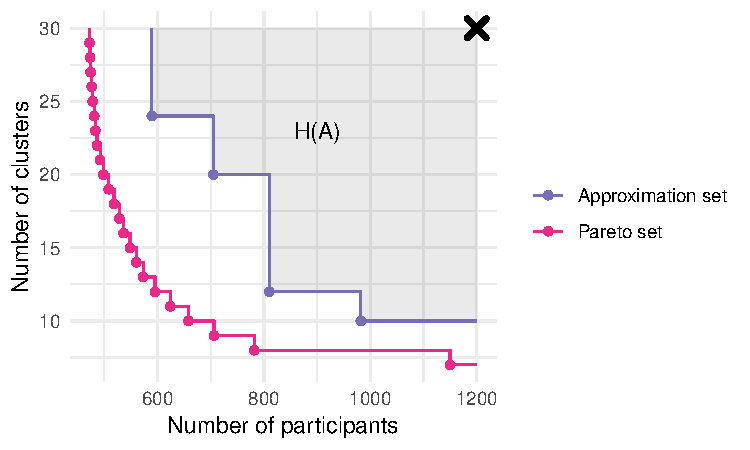
\includegraphics[scale=0.8]{./Figures/fake_pareto}
\caption{Example Pareto front $\mathcal{X}_{p}$ (green) and approximation set $\mathcal{A}$ (yellow) for a cluster randomised trial design problem. The dominated hypervolume of the approximation set with respect to a reference point (cross) is the shaded area.}
\label{fig:fake_pareto}
\end{figure}


\section{Simulation-based optimal trial design}\label{sec:methods}

We propose to apply the efficient global optimisation algorithm of~\cite{Jones1998}, also known as Bayesian optimisation, to solve trial design problems of the type described in Section~\ref{sec:examples}. This algorithm recognises that the evaluation of a solution is an expensive operation, and invests resources in carefully selecting each solution to be evaluated next. To do so, a non-parametric regression model approximating the true underlying function of interest is constructed and used to describe our knowledge and uncertainty about the true function value at solutions which have not yet been evaluated. Optimisation then proceeds in a probabilistic framework by considering a point $\textbf{x}_{*}$ for evaluation and asking questions such as `what is the probability that the solution $\textbf{x}$ is better than all the solutions I have evaluated so far?', and `how much of an improvement can I expect to see if I evaluate $\textbf{x}$?'. For clarity, we will focus here on the case where there is a single constraint function $g$, e.g. the power function, which must be evaluated using the Monte Carlo method. Algorithm~\ref{alg:EGO} describes the procedure.

\begin{algorithm}
\caption{Efficient Global Optimisation}\label{alg:EGO}
\begin{algorithmic}[1]
\State Compute MC estimates $\mathbf{y}_{E} = (g(\mathbf{x}^{(1)}), \ldots , g(\mathbf{x}^{(E)}))$
\While{Computation budget not exhausted}
\State Regress $\mathbf{y_{E}}$ on $\mathcal{X}_{E} = (\mathbf{x}^{(1)}, \ldots , \mathbf{x}^{(E)})$
\State Find $\mathbf{x}_{*} = \arg\max EI(\mathbf{x})$
\State Compute MC estimate $y_{*} = g(\mathbf{x}_{*})$ and add to $\mathbf{y_{E}},~\mathcal{X}_{E}$
\State Update the computational budget
\EndWhile
\end{algorithmic}
\end{algorithm}

In what follows we will first consider step (3), describing Gaussian process regression models and outlining how they can be fitted and used to make predictions. The notion of expected improvement ($EI$) in step (4) will then be defined for the constrained multi-objective problems we are concerned with. We then cover the remaining aspects of implementation.

%The algorithm is efficient in the sense that the number of evaluations of the expensive function is kept low - we will see later that problems can be solved with around 100 - 200 evaluations. However, note that in every iteration of the algorithm we must solve two other problems - the fitting of the regression model to the observed data (step 2), and the maximisation of expected improvement (step 3). The efficiency of this approach therefore rests on these problems being significantly easier to solve that the original SSD problem. Fortunately, both of these sub-problems are tractable if the regression model is a \emph{Gaussian process}. In the remainder of this section we will first describe Gaussian processes and show how they can be used to make predictions of expensive functions. We then describe the an efficient algorithm for the constrained, multi-objective, global optimisation problems of the type described in Section~\ref{sec:background}. Details of implementation are also be provided.

\subsection{Gaussian process regression}\label{sec:GP}

%Consider a set of $E$ points in the solution space, $\mathcal{X}_{E} = \{ \textbf{x}^{(1)}, \ldots , \textbf{x}^{(E)} \} \subset \mathcal{X}$, at which we plan to estimate a function $f$. The resulting data will then be used to predict the value of the function $f$ at another point $\mathbf{x}_{*}$. Here, we describe how such a prediction can be made using a Gaussian process model. More details on Gaussian processes can be found in~\cite{Rasmussen2006}.

%A Gaussian process (GP) is a collection of random variables, any finite number of which have a joint Gaussian distribution~\cite{Rasmussen2006}. A GP over $\mathcal{X}$ can be interpreted as representing our knowledge and uncertainty about the true value of $f$. 

Consider a set of points $\mathcal{X}_{E} = \{ \textbf{x}^{(1)}, \ldots , \textbf{x}^{(E)} \} \subset \mathcal{X}$ at which an expensive function $g$ will be estimated using the Monte Carlo method. Consider also some other point $\mathbf{x}_{*} \not\in \mathcal{X}_{E}$ where we are interested in making a prediction of $g(\mathbf{x}_{*})$. The value of $g$ at each point in $\{\mathcal{X}_{E}, \mathbf{x}_{*}\}$ is initially unknown, but can be modelled by a Gaussian process (GP). 

In using a GP we assume that our belief regarding the the values of $g$ can be represented as a multivariate normal distribution. Prior to computing any estimates of $g$, we assume that the mean function of this multivariate normal is equal to zero\footnote{This is not a restrictive assumption. After observing estimates of the function $g$ and updating the GP model to account for these, the mean function can take on non-zero values.}.
We write the (symmetric, positive definite) covariance matrix of the distribution as
\begin{equation}\label{eqn:cov_matrix}
\begin{pmatrix}
K(\mathcal{X}_{E}, \mathcal{X}_{E}) & K(\mathcal{X}_{E}, \mathbf{x}_{*}) \\
K(\mathbf{x}_{*}, \mathcal{X}_{E}) & K(\mathbf{x}_{*}, \mathbf{x}_{*})
\end{pmatrix}.
\end{equation}
$K(\mathcal{X}_{E}, \mathcal{X}_{E})$ is the $E \times E$ covariance matrix for the points $\mathcal{X}_{E}$, $\mathbf{k}_{*} = K(\mathcal{X}_{E}, \mathbf{x}_{*})$ is the $E$-length vector of covariances between $\mathcal{X}_{E}$ and $\mathbf{x}_{*}$, and $K(\mathbf{x}_{*}, \mathbf{x}_{*})$ is the variance at $\mathbf{x}_{*}$.

Given this prior distribution, we compute the MC estimates $y^{(1)} , \ldots , y^{(E)}$ at each point in $\mathcal{X}_{E}$. From equation (\ref{eqn:MC_error}), $y^{(i)} = g(\textbf{x}^{(i)}) + e^{(i)}$ where $e^{(i)}$ is a zero-mean normally distributed error term with standard deviation $\omega^{(i)}$. We denote by $\Delta$ the $E \times E$ diagonal matrix where the $i$th entry is $[\omega^{(i)}]^{2}$. The distribution of $g(\mathbf{x}_{*})$ conditional on the observed $\mathbf{y}$ can be shown to be normal with mean $\mathbf{k}_{*}^\top(K + \Delta)^{-1}\mathbf{y}$ and variance $k(x_{*}, x_{*})-\mathbf{k}_{*}^\top(K + \Delta)^{-1}\mathbf{k}_{*}$~\cite{Rasmussen2006}. Thus, given a prior covariance matrix of the form (\ref{eqn:cov_matrix}) and some MC estimates of $g$ at the points $\mathcal{X}_{E}$, a conditional predictive distribution of $g(\mathbf{x}_{*})$ can be found. It is this distribution which will be used in the optimisation algorithm when deciding which solution should next be evaluated.

The predictive distributions are influenced by the prior covariance matrix (\ref{eqn:cov_matrix}). The matrix is populated using a covariance function (or \emph{kernel}), $k(\mathbf{x}, \mathbf{x}') : \mathcal{X} \times \mathcal{X} \rightarrow \mathbb{R}$. This function must be symmetric and positive definite for the covariance matrix to have the same properties. One such covariance function is the squared exponential, which has the form
\begin{equation}
k(\mathbf{x}, \mathbf{x}') = \sigma \exp \left( -\sum_{j=1}^{D} \frac{(x_{j} - x'_{j})^2}{\lambda_{j}^2} \right).
\end{equation}
By using covariance functions of this form we will obtain a Gaussian process which is infinitely differentiable over $\mathcal{X}$ and thus very smooth. This would appear to be a reasonable restriction to place upon the power functions we are interested in. In order to populate the covariance matrix we must choose values of the hyper-parameters $\boldsymbol{\theta} = (\sigma, \lambda_{1}, \ldots, \lambda_{D})$. We do this by numerically optimising the log marginal likelihood
\begin{equation}\label{eqn:loglik}
\log{p(\mathbf{y} \mid \mathcal{X}_{E}, \boldsymbol{\theta})} = -\frac{1}{2}\mathbf{y}^\top[K + \Delta]^{-1}\mathbf{y} - \frac{1}{2} \log{|K + \Delta|} - \frac{n}{2} \log{2\pi},
\end{equation}
considered as a function of $\boldsymbol{\theta}$~\cite{Rasmussen2006}. Fitting a GP model by maximum likelihood in this manner can be done using the function \texttt{km} in the R package DiceKriging, as illustrated in the appendix.

An illustration of a Gaussian process regression model of a power function in one dimension is given in Figure~\ref{fig:GP_example}. The power of three different choices of sample size have been calculated and a GP model fitted to the results. The figure illustrates how the uncertainty in the model predictions (shaded area) increases the further we are from a point which has been evaluated. The GP prediction of power at a sample size of $n = 190$, shown as a dashed line, is normally distributed with mean 0.84 and standard deviation 0.035.

\begin{figure}
\centering
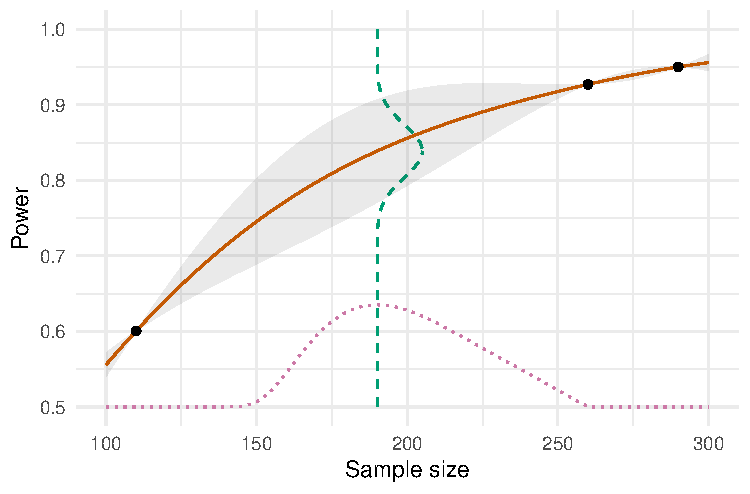
\includegraphics[scale=0.8]{./Figures/GP_example}
\caption{A Gaussian process model of a power function over a one-dimensional sample size (solid line) based on three evaluations. Uncertainty is shown as the shaded area. Expected improvement (dotted line) is maximised at a sample size of 190, where the predicted power is normally distributed around a mean estimate of 0.84 (dashed line).}
\label{fig:GP_example}
\end{figure}

%This optimisation can be assisted by using derivatives, which are available in closed form~\cite{Rasmussen2006}. The calculation of the log marginal likelihood involves the inversion of an $E \times E$ matrix, an operation which requires $\mathcal{O}(E^{3})$ time. In the problems we are interested in $E$ will typically be in the order of hundreds, meaning the calculation of (\ref{eqn:loglik}) is fast and thus the maximum likelihood optimisation remains tractable.

%The optimisation of $\boldsymbol{\theta}$ may involve several local minima, and so there is no guarantee that the solution produced by a numerical optimiser will be the globally optimal solution. It is therefore recommended that the resulting mean function of the conditional distribution over $\mathcal{X}$ is examined graphically to ensure it broadly aligns with prior expectations. Another way to test the quality of the fitted Gaussian process is to predict the value of $f$ at an unobserved point $\mathbf{x}_{*}$, and compute an MC estimate at that point for comparison. This can be done over the course of the efficient global optimisation algorithm (EGO), which we describe in the following section.

\subsection{Expected improvement}\label{sec:EGO}

At any given point during the optimisation process we can obtain an approximation set $\mathcal{A}$ based on the set of solutions which have been evaluated up to that point. If a new point $\mathbf{x}_{*}$ is considered feasible, a new approximation set $\mathcal{A}_{*}$ will be identified. The improvement resulting from the evaluation of $\mathbf{x}_{*}$ is the difference in the dominated hypervolumes:
\begin{equation}
I = H(\mathcal{A}_{*}) - H(\mathcal{A}).
\end{equation}

Prior to evaluation, we do not know if the point $\mathbf{x}_{*}$ will be considered feasible. We therefore modify $I$ to account for the probability that $\mathbf{x}_{*}$ will be considered feasible after the MC estimates have been obtained. This probability can be estimated using the GP regression methodology described in Section~\ref{sec:GP}. A GP model of unknown constraint function $g$ will give a prediction $g(\mathbf{x}_{*}) \sim \mathcal{N}(m, s^{2})$, and we will consider the point $\mathbf{x}_{*}$ feasible if the upper $100 \times p$\% quantile of this distribution is below 0. We denote this quantile as
\begin{equation}\label{eqn:quant}
q(\mathbf{x}_{*}) = m + \Phi^{-1}(p)s,
\end{equation}
where $\Phi$ is the standard normal cummulative distribution. Following an evaluation of $\mathbf{x}_{*}$ the GP model will be updated and the quantile revised to $q_{+}(\mathbf{x}_{*})$. Before the evaluation the value of $q_{+}(\mathbf{x}_{*})$ is unknown, but it is shown in~\cite{Picheny2014} that its predictive distribution is $q_{+}(\mathbf{x}_{*}) \sim N(m_{+}, s_{+}^{2})$ where
\begin{align}
m_{+} &= m + \Phi^{-1}(p)\sqrt{\frac{\omega^{2}s^{2}}{\omega^{2} + s^{2}}} \\
s_{+}^{2} &= \frac{[s^{2}]^{2}}{\omega^{2} + s^{2}},
\end{align}
and $\omega$ is the MC error of the planned evaluation, estimated as $m(1-m)/N$ where $N$ is the number of MC samples to be used. The predictive distribution can then be used to calculate the probability that the point $\mathbf{x}_{*}$ will be considered feasible following its evaluation. Following~\cite{Sasena2002}, we multiply the theoretical improvement $I$ by this probability, thus penalising candidate solutions with a low chance of satisfying the constraint. We then choose to evaluate the solution which maximises
\begin{equation}
EI = [H(\mathcal{A}_{*}) - H(\mathcal{A})] \prod_{j=1}^{C} \Phi\left(\frac{-m_{j,+}}{s_{j,+}}\right),
\end{equation}
where we now include all $j = 1, \ldots , C$ constraint functions. This maximisation problem is in itself complex, with a potentially large number of local maxima. We therefore use the particle swarm optimisation algorithm as implemented in the R package pso~\cite{Bendtsen2012}, designed to avoid becoming trapped in local maxima, to solve this sub-problem.

An illustration of expected improvement for a single-objective problem is given in Figure~\ref{fig:GP_example}. When choosing which sample size to evaluate next and aiming to find the lowest sample size with at least 80\% power, we balance the potential improvement over the best current solution (a sample size of 260) with the probability of constraint satisfaction. In this case, we would choose to evaluate the sample size of 190, estimated by the GP model to have a power of 84\%.

\subsection{Implementation}

To apply Algorithm~\ref{alg:EGO} in practice we must first choose the initial set of points to be evaluated, $\mathcal{X}_{E}$. One recommendation is to include 10 points for each dimension of the solution space, and to allocate between 25 and 50\% of the total computation budget to their evaluation~\cite{}. To select the location of the points in $\mathcal{X}_{E}$ we use a random Latin hypercube sample generated using the R package lhs~\cite{Carnell2016}, with the sample optimised to maximise the minimum distance between the points. The number of iterations and the number of MC samples $N$ used at each iteration must also be chosen. Given a total computational budget in terms of MC samples, the choice of these values should account for the fact that fitting GP regression models in R to more than around 800 points is infeasible~\cite{Chevalier2014}. 

As the algorithm depends on GP regression models, it is important that the fit of these models is assessed. One approach is to regularly plot the predicted mean and standard deviation in one dimension, centred at the last evaluated point. Poor model fit could be identified if the mean function is not, for example, strictly increasing as expected. We can also contrast the predicted function values with the obtained function values at each iteration, halting the algorithm if a large and unexpected discrepancy in these values is observed.

We have used R to implement the proposed framework, partly due to the availability of robust and efficient R packages for fitting Gaussain process models (DiceKriging~\cite{Roustant2012}) and for global optimisation (pso~\cite{Bendtsen2012}). Using R also provides flexibility in terms of the user-writen simulation routines by facilitating various complicated analysis procedures, e.g. multilevel modelling through lme4~\cite{Bates2015}. Our implementation works to a simple interface. The user must provide instances of three data frames. The first, \texttt{sol\char`_space}, contains a row for each design parameter describing its name and its lower and upper bounds. The second, \texttt{hypotheses}, contains a row for each hypothesis which power is to be simulated under. Each row should include a label and a value for each parameter needed (together with design parameters) to define the simulation. Finally, \texttt{constraints} contains a row for each constraint function $g_{j}$. Each row should include a label for the constraint, the hypothesis it pertains to, a nominal power which should not be exceeded, and the confidence we require in the constraint being satisfied (i.e. the $p$ in Equation~\ref{eqn:quant}). Further, two functions are required. The first, \texttt{objectives}, takes as argument a vector of design parameter values $\mathbf{x}$ and returns a vector of objective values $( f_{1}(\mathbf{x}), \ldots, f_{B}(\mathbf{x}) )$. The second, \texttt{sim\char`_trial}, takes as arguments a vector of design parameter values $\mathbf{x}$ and a hypothesis (i.e. a row from the hypotheses data frame). The function should simulate the necessary data generation and analysis and return a boolean indicator of the rejection of the null hypothesis, or, more generally, of declaring `success'. Given these components, the example R code in the appendix can be modified to solve the trial design problem at hand.

\section{Application to the examples}\label{sec:application}

\subsection{Cross-classified psychotherapy trial}

Recall our first motivating example of a cross-classified psychotherapy trial. The design parameters are the number of participants in the intervention arm $n_{2}$, the between-arm allocation ration $r$, the number of therapists $k$ and the number of doctors $j$. For simplicity and ease of illustration we will fix $j = 50$. The bounds on the remaining design parameters are taken to be $r \in [0.5, 1]$, $n_{2} \in [200, 1000]$, and $k \in [5, 40]$. 
%This defines the solution space $\mathcal{X} = \{(r, n_{2}, k) \mid r \in [0.5, 1] \subset \mathbb{R}, n_{2} \in [200, 1000] \subset \mathbb{Z}, k \in [5, 40] \subset \mathbb{Z} \}$.

%, \sigma_{w}^{2} = 0.96, \sigma_{d}^{2} = 0.03, \sigma_{t}^{2} = 0.01

We wish to minimise both the total number of patients $f_{1}(\mathbf{x}) = (r+1)n_{2}$ and the number of therapists $f_{2}(\mathbf{x}) = k$. The only constraint we must satisfy is that the type II error rate $\beta(\mathbf{x})$ under the alternative hypothesis $H_{1}: \beta_{1} = 0.3$ is no more than $\beta^{*} = 0.2$. This gives the constraint function $g_{1}(\mathbf{x}) = \beta(\mathbf{x}) - 0.2$. A program to simulate the data generation and analysis under $H_{1}$ for a given $\mathbf{x}$ is given in the appendix.

We initialised the optimisation algorithm by generating a random Latin hypercube sample of size 30 and computing MC estimates of power for each point using $N = 250$ samples. Following this, 60 iterations of Algorithm~\ref{alg:EGO} were applied, with $N = 500$ samples used at each iteration. In Figure~\ref{fig:CC_single_run} we plot the 90 evaluated solutions in the objective space, distinguishing between those in the initial design $\mathcal{X}_{E}$, those which where subsequently evaluated during the iterative phase of the algorithm, and those which together form the final approximation set.

\begin{figure}
\centering
\includegraphics[scale=0.8]{./Figures/CC_single_run}
\caption{Objective values of solutions in the initial set $\mathcal{X}_{E}$ (blue), subsequent iterations of the algorithm (green), and those in the final approximation of the Pareto set (yellow).}
\label{fig:CC_single_run}
\end{figure}

At the $i$th iteration of the algorithm we calculated the dominated volume $H(\mathcal{A}_{i})$, plotted in Figure~\ref{fig:CC_traj}. Also plotted is the expected improvement, calculated at iteration $i$ with respect to iteration $i+1$, and the subsequent prediction of the dominated volume $H(\mathcal{A}_{i+1})$. In this instance the algorithm appears to plateau after around 40 iterations. Note that $H(\mathcal{A}_{i})$ is not strictly increasing. This is because the evaluation of a new solution can lead to revised estimates of other solutions which were in the approximation set, such that they are then considered infeasible and removed from the set. 

\begin{figure}
\centering
\includegraphics[scale=0.8]{./Figures/CC_traj}
\caption{Quality of the approximation set obtained as the algorithm proceeds (solid line). The maximised expected improvement at each iteration is also plotted (dashed line), together with the corresponding predicted approximation set quality (dotted line).}
\label{fig:CC_traj}
\end{figure}

The solutions which form the final approximation set are detailed in Table~\ref{tab:CC_single_run}. As few as 9 therapists can lead to a sufficiently powered trial, although nearly 1000 participants are required in this configuration. On the other hand, if minimising the total sample size is deemed more important than minimising the number of therapists, we see that as few as 535 participants are necessary providing 27 therapists are included. The approximation set contains 13 solutions in total, providing a reasonable set of options from which the solution best representing the priorities of the decision maker(s) can be selected.

\begin{table}
\centering
\begin{tabular}{rrrrrr}
\toprule
$r$ & $n_{2}$ & $k$ & $\hat{\beta}~(s.e.)$ & $f_{1}$ & $f_{2}$ \\ 
\midrule
0.87 & 286 & 27 & 0.178 (0.017) & 535 & 27 \\ 
0.85 & 299 & 26 & 0.200 (0.018) & 553 & 26 \\ 
0.82 & 316 & 25 & 0.178 (0.017) & 575 & 25 \\ 
0.83 & 321 & 24 & 0.166 (0.017) & 587 & 24 \\ 
0.82 & 334 & 23 & 0.188 (0.017) & 609 & 23 \\ 
0.82 & 356 & 21 & 0.208 (0.018) & 648 & 21 \\ 
0.85 & 362 & 15 & 0.168 (0.017) & 669 & 15 \\ 
0.83 & 375 & 14 & 0.172 (0.017) & 687 & 14 \\ 
0.85 & 377 & 13 & 0.214 (0.018) & 696 & 13 \\ 
0.87 & 394 & 12 & 0.166 (0.017) & 735 & 12 \\ 
0.88 & 412 & 11 & 0.180 (0.017) & 775 & 11 \\ 
0.92 & 442 & 10 & 0.168 (0.017) & 847 & 10 \\ 
0.92 & 513 & 9 & 0.176 (0.017) & 986 & 9 \\ 
\bottomrule
\end{tabular}
\caption{Approximation set after 60 iterations of Bayesian optimisation for the cross-classified design problem. Solutions are defined by their allocation ratio $r$, sample size in the intervention arm $n_{2}$, and number of therapists $k$. Type II error rate $\beta$ is constrained to be below 0.2, while the total sample size $f_{1}$ and number of therapists $f_{2}$ are to be minimised.}
\label{tab:CC_single_run}
\end{table}

%9th solution - raw MC estimate of 0.214 (s.e. = 0.018), upper CI 0.257. But GP model gives 0.185 (0.005), upper CI 0.196. MC estimate with 10,000 samples gives: 0.1844 (0.003878295), upper CI 0.193.

As can be seen from Table~\ref{tab:CC_single_run}, approximate upper 99\% confidence limits based on the MC estimates of power often exceed the corresponding nominal bound of 0.2. For example, the solution described in the last row would have an approximate 98\% two-sided confidence interval of $(0.172, 0.256)$ . However, when the GP model is used to predict power instead of the raw MC estimate, the interval is $(0.173, 0.197)$.  To verify this prediction we computed a more precise MC estimate using $N = 10,000$ samples, which gave an interval of $(0.175, 0.193)$.

\subsection{Cluster-randomised pilot trial}

Recall our second motivating example, the cluster randomised pilot trial in care homes. In this case we have 6 design parameters to optimise over: the numbers of clusters in each arm, $k_{1}$ and $k_{2}$; the cluster size in each arm, $m_{1}$ and $m_{2}$; and the critical region adjustments for the tests of response and adherence, $c_{r}$ and $c_{a}$. 
%Together with their bounds they specify the solutions space
%\begin{equation}
%\mathcal{X} = \{ (m_{1}, k_{1}, m_{2}, k_{2}, c_{a}, c_{r}) \mid m_{1}, m_{2} \in [5,25] \subset \mathbb{Z}, k_{1}, k_{2} \in [3,15] \subset \mathbb{Z}, c_{r}, c_{a} \in [-2,2] \subset \mathbb{R} \}.
%\end{equation}
As in the preceding example, the objective space has two dimensions. We aim to minimise the total number of participants $f_{1}(\mathbf{x}) = m_{1}k_{1} + m_{2}k_{2}$ and the total number of clusters $f_{2}(\mathbf{x}) = k_{1} + k_{2}$. In this example we have three constraint functions: $g_{1}(\mathbf{x}) = \alpha_{r}(\mathbf{x}) - 0.3$; $g_{2}(\mathbf{x}) = \alpha_{a}(\mathbf{x}) - 0.4$; and $g_{3}(\mathbf{x}) = \beta(\mathbf{x}) - 0.1$. Again, a program for the simulation of the trial data generation and analysis is given in the appendix.

A 60-point Latin hypercube sample $\mathcal{X}_{E}$ of initial solutions was generated, and these were evaluated using $N = 250$ MC samples. Following this, 60 iterations of Bayesian optimisation were then applied, using $N = 500$ samples for each MC estimate. The resulting approximation set is illustrated in Figure~\ref{fig:pilot_single_run}, together with some of the initial set $\mathcal{X}_{E}$ and the solutions evaluated during the iterative phase of the algorithm.

\begin{figure}
\centering
\includegraphics[scale=0.9]{./Figures/pilot_single_run}
\caption{Going up to 60 iterations. We have focussed on the approximation set, omitting 34 points (all from the initial design) which take larger values of $f_{1}$ and/or $f_{2}$. }
\label{fig:pilot_single_run}
\end{figure}

\begin{figure}
\centering
\includegraphics[scale=0.9]{./Figures/pilot_traj}
\caption{Quality of the approximation set obtained as the algorithm proceeds (solid line). The maximised expected improvement at each iteration is also plotted (dashed line), together with the corresponding predicted approximation set quality (dotted line).}
\label{fig:pilot_traj}
\end{figure}

Only 12 of the initial 60 solutions are displayed in Figure~\ref{fig:pilot_single_run}, with the remainder being located outwith the plotted range. The final solutions which form the approximation set are described in further detail in Table~\ref{tab:pilot_single_run}. The results suggests that at least 6 clusters are required in total. Reducing the total number of participants required from 144 to 95 is possible, providing an increase in the number of clusters from 6 to 13 is deemed acceptable. The approximation set contains 5 solutions in total, which, given the scales involved, would appear to provide sufficient flexibility to enable a trial design with the desired balance between objectives to be found.

\begin{table}
\centering
\begin{tabular}{rrrrrrrrrrrrrrrr}
\toprule 
$m_{1}$ & $k_{1}$ & $n_{1}$ & $m_{2}$ & $k_{2}$ & $n_{2}$ & $c_{r}$ & $c_{a}$ & $\hat{\beta}~(s.e.)$ & $\hat{\alpha}_{r}~(s.e.)$ & $\hat{\alpha}_{a}~(s.e.)$ & $f_{1}$ & $f_{2}$ \\
\midrule
5 & 8 & 40 & 10 & 6 & 60 & 0.094 & -0.013 & 0.092 (0.013) & 0.270 (0.020) & 0.328 (0.021) & 100 & 14 \\ 
6 & 6 & 36 & 11 & 6 & 66 & 0.086 & -0.036 & 0.084 (0.012) & 0.234 (0.019) & 0.310 (0.021) & 102 & 12 \\ 
8 & 5 & 40 & 12 & 6 & 72 & 0.104 & -0.050 & 0.080 (0.012) & 0.288 (0.020) & 0.286 (0.020) & 112 & 11 \\ 
10 & 4 & 40 & 13 & 6 & 78 & 0.068 & -0.099 & 0.092 (0.013) & 0.266 (0.020) & 0.294 (0.020) & 118 & 10 \\ 
19 & 3 & 57 & 23 & 3 & 69 & 0.121 & 0.084 & 0.110 (0.014) & 0.262 (0.020) & 0.344 (0.021) & 126 & 6 \\ 
\bottomrule
\end{tabular}
\caption{Approximation set after 60 iterations of Bayesian optimisation for the pilot trial design problem.
Solutions are defined by the number of clusters $k_{i}$ and participants per cluster $m_{i}$ for each arm $i=1,2$, together with critical region adjustments $c_{r}, c_{a}$. The total number of participants $f_{1}$ and number of clusters $f_{2}$ are to be minimised, subject to constrained error rates $\beta < 0.1, \alpha_{r} < 0.3$ and $\alpha_{a} < 0.4$.}
\label{tab:pilot_single_run}
\end{table}

%last solution - raw MC estimate of 0.110 (s.e. = 0.014). But GP model gives 0.08772435 (0.004699269), MC estimate with 10,000 samples gives: 0.0949 (0.002930914)

As can be seen from Table~\ref{tab:pilot_single_run}, approximate upper 98\% confidence limits for the MC power estimates often exceed the corresponding nominal bound. For example, the last solution given would have an approximate 98\% two-sided confidence interval of $(0.078, 0.143)$ . However, when the GP model is used to predict power instead of the raw MC estimate, the interval is $(0.077, 0.099)$.  To verify this prediction we computed a more precise MC estimate using $N = 10,000$ samples, which gave a interval of $(0.088, 0.102)$.

\section{Simulation study}\label{sec:simulation}

Algorithm~\ref{alg:EGO} is stochastic and will return a different final approximation set each time it is applied to the same problem. To assess the variability in the quality of these sets, we conducted two simulation studies using the two illustrative examples of Section~\ref{sec:examples}. For each problem the algorithm was applied 1000 times. Each application was as described in Section~\ref{sec:application}, although now using 200 iterations as opposed to 60. 

We recorded the approximation sets $\mathcal{A}_{i}^{(j)}$ found at iteration $i \in [1,200]$ for each run $j \in [1,1000]$. Recall that the quality of an approximation set $\mathcal{A}_{i}^{(j)}$ is measured by the volume of the dominated subspace $H(\mathcal{A}_{i}^{(j)})$ as compared with that of the Pareto set $\mathcal{X}_{p}$:
\begin{equation}
H(\mathcal{X}_{p}) - H(\mathcal{A}_{i}^{(j)}),
\end{equation}
As $\mathcal{X}_{p}$ is unknown, we instead use the set of non-dominated solutions in the union of the final approximation sets produced by the 1000 applications of the algorithm, $\mathcal{X}_{p} \approx \cup_{j=1}^{1000} \mathcal{A}_{200}^{(j)}$.

For comparison, we implemented an alternative method based on a fixed experimental design. To compare against the algorithm after $i$ iterations, the average time taken to reach iteration $i$ over the 1000 runs was calculated. The number of solution evaluations (using $N = 500$ MC samples) which could be completed in this time was then found. A fixed space-filling experimental design\footnote{We used a Sobol sequence, which has the convenient property that the sequence of size $i+1$ contains the sequence of size $i$ for all $i > 0$.}
of this size, $\mathcal{X}_{d}$, was then generated. For each problem, the set $\mathcal{X}_{d}$ was chosen from a restricted region of the full solution space. Specifically, in the cross-classified example we restricted solutions to those with balance between the arms, i.e. $r=1$, and in the pilot trial example to those with balance between arms and clusters, i.e. $m_{1} = m_{2}$ and $k_{1} = k_{2}$. These simple heuristics were designed to allow the set $\mathcal{X}_{d}$ to more fully explore the fundamental parameters of total sample size and total number of clusters.

Each solution in $\mathcal{X}_{d}$ was evaluated using $N=500$ samples. Approximate 98\% two-sided confidence intervals for each constraint function value were calculated. As with Algorithm~\ref{alg:EGO}, a constraint was considered to be satisfied if the upper confidence interval was within the nominal bound. The approximation set of non-dominated feasible solutions was then identified.

\subsection{Cross-classified psychotherapy trial}

Figure~\ref{fig:CC_hv_iters} illustrates the distribution in the quality of approximation sets found at different stages of the optimisation algorithm. Both variability and median dominated hypervolume reduce steadily as the number of iterations increases, with the rate of change being most extreme in the initial stages of the search. Before the iterative portion of the optimisation algorithm starts, the majority of runs return approximation sets of worse quality than the matched fixed design method. However, as the number of iterations increase the optimisation algorithm consistently out-performs the fixed experimental design method. 

\begin{figure}
\centering
\includegraphics[scale=0.9]{./Figures/CC_hv_iters}
\caption{Box plots illustrating the differences in dominated hypervolumes obtained as the number of iterations in the Bayesian optimisation algorithm increases. Corresponding differences obtained using the fixed experimental design are shown in red.}
\label{fig:CC_hv_iters}
\end{figure}

\begin{figure}
\centering
\includegraphics[scale=0.9]{./Figures/CC_ex_0}
\caption{Random selection of approximation fronts obtained after 0 iterations of the Bayesian optimisation algorithm (coloured lines) for the cross-classified problem, together with the Pareto front (dashed black line) and the approximation front obtained using the fixed experimental design (solid black line). Time taken - 1 hr 2 mins.}
\label{fig:CC_ex_0}
\end{figure}

A random selection of 10 approximation fronts with 0 iterations completed is illustrated in Figure~\ref{fig:CC_ex_0}. The approximation sets from the same 10 runs are shown again in Figure~\ref{fig:CC_ex_60}, now after 60 iterations of the optimisation algorithm. Average quality has clearly increased, although at the cost of computation time - on average, 4 hours and 38 minutes were required to reach 60 iterations, whereas 1 hour and 2 minutes were needed to evaluate the initial experimental design. However, note that the benefits of the Bayesian optimisation algorithm over the fixed experimental design become clear by this point. Comparing the approximation set of the first run (bold red in Figure~\ref{fig:CC_ex_60}) with that of the fixed design in terms of the numbers of participants required (i.e. objective $f_{1}$), we see that the algorithm requires between 24 and 396 fewer participants for the same number of therapists. Moreover, it provides solutions requiring as few as 6 therapists, whereas the fixed design does not provide an option for less than 7. As the number of iterations increases to 200, illustrated in Figure~\ref{fig:CC_ex_200}, the average computation time increases to over 13 hours but the improvement in solution quality is limited.

\begin{figure}
\centering
\includegraphics[scale=0.9]{./Figures/CC_ex_60}
\caption{Random selection of approximation fronts obtained after 60 iterations of the Bayesian optimisation algorithm (coloured lines) for the cross-classified problem, together with the Pareto front (dashed black line) and the approximation front obtained using the fixed experimental design (solid black line).}
\label{fig:CC_ex_60}
\end{figure}

\begin{figure}
\centering
\includegraphics[scale=0.9]{./Figures/CC_ex_200}
\caption{Random selection of approximation fronts obtained after 200 iterations of the Bayesian optimisation algorithm (coloured lines) for the cross-classified problem, together with the Pareto front (dashed black line) and the approximation front obtained using the fixed experimental design (solid black line).}
\label{fig:CC_ex_200}
\end{figure}

%We set $r = 1$ to simplify the SSD - quantiles for the optimal results across all runs give quantiles
%       0%       25%       50%       75%      100% 
%0.6103892 0.9077041 0.9761386 1.0000000 1.0000000 
%, so seems about right.

\subsection{Cluster-randomised pilot trial}

We now consider the second motivating example. The quality of approximation sets, for increasing number of iterations, is plotted in Figure~\ref{fig:pilot_hv_iters}. The results of the fixed experimental design are shown for comparison.

\begin{figure}
\centering
\includegraphics[scale=0.9]{./Figures/pilot_hv_iters}
\caption{Box plots illustrating the differences in dominated hypervolumes obtained as the number of iterations in the Bayesian optimisation algorithm increases. Corresponding differences obtained using the fixed experimental design are shown in red.}
\label{fig:pilot_hv_iters}
\end{figure}

At the start of the iterative portion of the Bayesian optimisation algorithm, Figure~\ref{fig:pilot_hv_iters} shows substantial variability in the quality of the approximation set obtained. A random selection of 10 approximation fronts with 0 iterations completed is illustrated in Figure~\ref{fig:pilot_ex_0}.

\begin{figure}
\centering
\includegraphics[scale=0.9]{./Figures/pilot_ex_0}
\caption{Random selection of approximation fronts obtained after 0 iterations of the Bayesian optimisation algorithm (coloured lines), together with the Pareto front (dashed black line) and the approximation front obtained using the fixed experimental design (solid black line).}
% Time taken - 19 mins (on average).
\label{fig:pilot_ex_0}
\end{figure}

The quality of solutions increases substantially as the number of iterations is increased, with the rate of improvement levelling off quickly. The approximation sets from the same 10 runs of Figure~\ref{fig:pilot_ex_0} are shown again in Figure~\ref{fig:pilot_ex_60}, now after 60 iterations of the optimisation algorithm. Average quality has clearly increased, although at the cost of computation time - on average, 2 hours and 45 minutes were required to reach 60 iterations, whereas only 19 minutes were needed to evaluate the initial experimental design. However, note that the benefits of the Bayesian optimisation algorithm over the fixed experimental design are clear. Comparing the approximation set of the first run (bold red in Figure~\ref{fig:pilot_ex_60}) with that of the fixed experimental design in terms of the numbers of participants required, we see that the optimisation algorithm leads to solutions which require between 14 and 48 fewer participants for the same number of clusters. Moreover, it provides solutions requiring as few as 6 clusters, whereas the fixed design does not provide options for fewer than 8. As the number of iterations increases to 200, illustrated in Figure~\ref{fig:pilot_ex_200}, the average computation time increases to over 9 hours but the improvement in solution quality is limited.

\begin{figure}
\centering
\includegraphics[scale=0.9]{./Figures/pilot_ex_60}
\caption{Random selection of approximation fronts obtained after 60 iterations of the Bayesian optimisation algorithm (coloured lines), together with the Pareto front (dashed black line) and the approximation front obtained using the fixed experimental design (solid black line).}
\label{fig:pilot_ex_60}
\end{figure}

\begin{figure}
\centering
\includegraphics[scale=0.9]{./Figures/pilot_ex_200}
\caption{Random selection of approximation fronts obtained after 200 iterations of the Bayesian optimisation algorithm (coloured lines), together with the Pareto front (dashed black line) and the approximation front obtained using the fixed experimental design (solid black line).}
\label{fig:pilot_ex_200}
\end{figure}


\section{Discussion}\label{sec:discussion}

Simulation-based design is often required for complex trials, yet the associated computational burden has led to the associated optimal design problems being simplified to enable a timely solution. These simplifications include fixing a number of design parameter values so that optimisation can take place over a single dimension and with respect to a single objective. Methods and associated software for simulation-based design are available for such problems~\cite{Landau2013, Hooper2013}, but the more general case has yet to be addressed. In this paper we have explored how surrogate models of operating characteristics and associated algorithms for efficient global optimisation can be used to facilitate simulation-based design of clinical trials where there are several parameters to be chosen, several objectives to minimise, and several constraints to satisfy.

The general optimisation framework we have suggested recognises that in many complex trials we are interested in minimising more than one quantity subject to constraints on operating characteristics. Problems of this sort are common in multilevel trial design~\cite{Hemming2017}, but are typically approached by first reducing the multiple objectives down to a single objective. For example, in the design of a cluster randomised trial it is common to fix the number of participants per cluster and minimise the number of clusters~\cite{Donner2000}, or vice-versa~\cite{Hemming2011, Eldridge2015}. Alternatively, a function which specifies the cost of sampling at the cluster and the patient level could be specified~\cite[p. 175]{Hox2002}, and the overall cost minimised~\cite{Snijders1993}. The latter approach has been suggested for both two-level~\cite{Raudenbush2000} and three-level hierarchical trial designs~\cite{Breukelen2012, Teerenstra2008}. However, the \emph{a priori} specification of such a cost function may not always be feasible, particularly when several stakeholders are involved. The Pareto optimisation framework we have described leads to a more computationally challenging optimisation problem, but produces solutions which will be more helpful to decision makers, enabling the available trade-offs between objectives to be seen and selected from. Multiple objectives have also arisen in adaptive designs, which can aim to minimise the expected sample size under several different hypotheses. Several authors have described methods for finding the Pareto set (or equivalently, the set of admissible designs) in this setting~\cite{Jung2001, Jung2004, Mander2012}, although without the use of benchmark multi-objective optimisation algorithms such as NSGA-II~\cite{Deb2002}.

%the methods used thus far have been inefficient, solving a large number of single-objective optimisation problems using different weighted combinations of objectives~\cite{Mander2012}. Using multi-criteria optimisation algorithms such as the benchmark NSGA-II~\cite{Deb2002}, as implemented in the R package mco~\cite{Mersmann2014}, would improve the efficiency of these methods.

%Comparison to alternative approaches

%MLPowSim and SimSam both do simulation based SSD, the former using a very simple grid (although this does lead to a multi-criteria solution of sorts), the latter is limited to problems in one dimension. Note that SimSam could have been used as part of the heuristic algorithm in Example 1 to improve its efficiency. 
%Many simulation SSD papers already do informal model-assisted design, by getting power at a set of $n$'s and drawing a line through the results.
%Our approach is very general, can be applied to pretty much any problem as long as we can simulate it and the number of design variables / criteria aren't too large (say, < 10).

%Implementation issues

%Reproducibility. Don't need to be able to repeat someone's SSD, but do want to be able to confirm the design they propose has the operating characteristics they claim. Will this mean people will have to make their simulation code freely available? If so, would want our software to be easy to use for this purpose. May connect with writing a simulation protocol as described in~\cite{Smith2010}.

As noted in Section~\ref{sec:intro}, related work in simulation-based design methodology has often focussed on a specific area of application. In this paper we have taken the view of~\cite{Hooper2013} and proposed a general framework which can be applied to almost any problem where the trial data generation and analysis can be simulated. It is argued in~\cite{Kontopantelis2016} that requiring the user to specify their own simulation program can be prohibitive in practice. One way to address this limitation is to share example programs for a range of problems, providing a starting point for the development of a new program. We have provided two such examples in the appendix.

When submitting a proposed design for approval by a funding body, it is important that the sample size calculation is transparent and replicable. When a simulation program has been used, supplying this as part of the application will help ensure this is the case. Given a copy of the program, any reviewer will be able to re-calculate the operating characteristics of the proposed design. However, a greater challenge is the validation of the program, where the program must be understood to ensure it is an accurate representation of the model in question. This requirement has partly motivated our use of R. Although significantly slower than a compiled language such as C++, it has been argued that software written in R is more transparent~\cite{Smith2010}. Validation will be further facilitated if a simulation protocol of the sort described in~\cite{Smith2010} is provided alongside the code. Nevertheless, to an applied statistician more familiar with alternative statistical software such as Stata or SAS, understanding and using an R program may require significant time and effort. Future work could focus on developing an interface with these statistical languages, allowing a simulation program to be written in them and connect with the R implementation of the optimisation algorithm through a suitable interface.

The examples have demonstrated that the time required to converge to a high quality approximation set can be significant, of the order of hours. Given that the majority of computational effort is expended generating MC samples when evaluating solutions, it is important that these simulation programs are as efficient as possible. Code profiling, used to identify areas which are consuming the most resources and making them more efficient, should be conducted. Future work could focus on using more sophisticated methods for surrogate modelling and efficient optimisation, such as imposing monotonicity conditions as described in~\cite{Emmerich2011}, to further improve computation time.

We have followed the conventional approach to clinical trial design whereby constraints on operating characteristics are set and then a constrained optimisation problem is solved. In practice the constraints are not fixed in advance, but adjusted iteratively in response to the design requirements they produce. Such an iterative procedure will clearly further increase an already substantial computational burden for simulation-based design. However, note that a change to a constraint does not mean starting the design process again. Any simulation data generated can still be used when fitting the GP model(s). An interactive routine whereby the user adjusts the constraints in response to the observed design requirements could be developed.

We have chosen to model each constraint function using a separate GP regression model. An alternative approach is to specify a single GP model which jointly models all constraint functions simultaneously, known as `co-krigging'. However, it has been noted that this is prone to error and does not necessarily improve efficiency significantly~\cite{}. A further alternative is to incorporate constraints into objective functions as penalisation terms, after which GP models of the penalised objectives could be modelled and a unconstrained optimisation problem solved. Disadvantages of this approach include greater difficulty in interpreting the GP models and thus diagnosing a poor fit, and the fact that the resulting function being modelled will be less smooth, with a large step change over the region of the constraint boundary, which may be more challenging to model well. We could consider other regression methods other than GPs, including parametric models. However, other modelling approaches do not provide the formal quantification of uncertainty in prediction that is obtained when using GP models, and so are less amenable for use in global optimisation. 

Numerous extensions to the proposed approach can be considered. One argument for simulation-based design is the ease with which sensitvity to model assumptions, such as the value of nuisance parameters, can be assessed~\cite{Landau2013}. We have not considered such investigations in this paper. An extension to the methodology could consider how a systematic assessment of sensitivity to nuisance parameters could be conducted, given a proposed trial design. Such investigations fall under the heading of \emph{uncertainty quantification} and can be carried out using GP regression and associated techniques~\cite{Kennedy2001}. A further extension could consider Bayesian approaches to trial design, including hybrid Bayesian-frequentist assurances~\cite{OHagan2005} and fully Bayesian measures such as average coverage criterion~\cite{Cao2009}. Aside from very simple cases involving only conjugate analyses, evaluating these Bayesian criteria will generally require simulation~\cite{OHagan2005} and so optimal design may benefit from the efficient methods discussed here.

\section{Conclusion}

Efficient optimisation algorithms based on surrogate models of expensive operating characteristic functions can be used to solve complex problems of clinical trial design. By using these methods we can avoid making unrealistic simplifying assumptions at the trial design stage, both in terms of the statistical model underlying the trial and of the nature of the optimal trial design problem.

%Limitations and alternatives

%The proposed optimisation algorithm has a number of parameters which have to be chosen. We have made some suggestions, but for every new problem there will be different optimal choices. Further work and experience in applying the method to a wider range of problems may help in identifying good robust choices for these parameters.
%We have used GPs, but could consider other non-parametric regression models, e.g. splines, GAMs, etc. Key advantage of GPs is that they provide uncertainty in predictions, so good for sequential optimisation. Key limitation is the scaling with number of points, which in R makes models of more than 200 points quite slow.
%Could also consider parametric regression models, arguing that the power functions and expected sample size functions may have a form which we could guess at in advance. Although, can always add a model component to the GP and still get the flexibility when modelling the errors.
%When optimising the improvement criteria, we repeatedly get predictions of the GP models for just one point. We can get predicted values for many points at once with very little extra effort, which suggests a different algorithm which evaluates several points at once may be more efficient. Note that the pso we use does this, but we would need to write our own custom implementation to make it work for us.
%\cite{Knowles2006} gives an alternative way to do multi-objective EGO type optimisation

%Extensions

%Extension to Bayesian SSD. We have already cited~\cite{Wang2002}, also look at ``SAMPLE SIZE FOR BINOMIAL REGRESSION WITH MISCLASSIFICATION''.
%We have considered deterministic and cheap objective functions only. To tackle trial design problems with stochastic objectives which require simulation to evaluate, e.g. adaptive designs, we need to allow expensive stochastic objectives also.

%For both objective and constraint functions, we set the number of MC samples in the above calculations to the total computation budget available at that point. So, we choose the next point to evaluate assuming that we will use all our resources to do so. We actually use only a part of the budget, say $N = 1000$, before stopping and checking again if further evaluation is still warranted. This follows the strategy set out in~\cite{Picheny2010} for optimising noisy functions with on-line allocation of resources.

%\section{Conclusion}

\bibliographystyle{plain}
\bibliography{U:/Literature/Databases/DTWrefs}

\end{document}



















\section{Review}\label{sec:review}

\subsection{Power calculations and sample size determination by simulation}

%\cite{Feiveson2002} - Simple illustrations of how power can be estimated using simulation in Stata. No SSD.

%\cite{Wason2012} - For a MAMS design with a simple model, uses simulation since analytic methods don't work from more than 3 stages. Simulation is simple in the sense that only a multivariate normal test statistic is generated, not individual patient outcome. This is made possible by assuming variance is known - a more realistic model would give the type of computational burden we are interested in. Also, implemented in C so solution method not extendible to other designs. 

%\cite{Burton2006} General review of how simulation studies should be designed, conducted and reported. Not specific to SSD.

%\cite{Smith2010} Similar to Burton et al., a general overview of how a simulation study should be done in accordance with a protocol.

%\cite{Hooper2013} Heuristic algorithm for one dimensional SSD with simulation. Flexible interface, user writes the simulation. Slightly model-based heuristic.

%\cite{Landau2013} General strategy for simulation based SSD. Examples considered only one dimensional.

%\cite{Wang2002} Takes a Bayesian view, notes that we can use MC to evaluate some performance criteria in complex hierarchical models, and then choose the sample size to get the desired level of performance criteria. Only looks at one dimension, discretised. Emphasises the computational burden, meaning the approach may not be that useful in practice. 

%\cite{Baio2015} Focusses on stepped wedge SSD, reviewing some analytical formula and describing how simulation can be used to move past their limitations. The trial designs have three parameters (number of patients, number of clusters, number of observation time points) but only the number of patients is optimised over. Emphasises doing sensitivity analyses for the assumed parameters. Simulates power for some selected values of $n$ and then chooses the lowest which is powered. Suggests around 1000 MC simulations should be enough to estimate power. Includes a comparison of the analytic and simulation methods showing that in some cases the optimal sample sizes are different, so motivating the use of simulation. Has led to an R package "SWSamp"~\cite{} (see also Gianluca Baio's webpage) which uses the algorithm.

%\cite{Grieve2016} Focusses on sample size for logistic regression, and includes the approach of using simulation. Considers one dimensional problems. Starts by describing a bisection search. Then describes the SimSam algorithm. Applies Hooper's algorithm to three case studies.

%\cite{Hooper2016} Focuses on stepped wedge and longitudinal cluster trials. Gives analytical formulae and also described how SimSam can be used, so again only considers a one dimensional problem. Describes as a benefit of formulae over simulation the ability to see the effect of all the parameters - plots the design effect as we vary the cluster size, the ICC and another parameter. Discusses the problems arising from the necessary estimation of the extra parameters coming from these complex designs.

%\cite{Kontopantelis2016} Describes a Stata program ipdpower for sample size in two-level models using simulation, motivated by individual patient level meta-analysis. Mentions SimSam but states that the fact that the data generation model has to be manually specified as a disadvantage - so they are trying to develop something easier to use but less flexible. Doesn't actually do any optimisation, just power calcs, suggest that we can just do a bisection search using these.

%\cite{Schoenfeld2005} Provides an analytic method (an algorithm) for power and SSD for logistic and proportional hazards models. Notes that simulation is an alternative, but at that point too computationally intensive to be practical.

%\cite{Arnold2009} Focussing on the general use of simulation to estimate power, aimed at showing social scientists and epidemiologists who might not be as familiar as statisticians. SSD just by calculating power over a one dimensional range and then plotting. Emphasises the benfits of simulation over its flexibility, particularly that it forces us to be specific about the planned analysis.

%\cite{Shao2007} Group sequential t-tests. Notes that the critical values used in these tests are usually taken from a multivariate normal since the actual multivariate t distribution is too complex to handle. Uses MC estimates of error rates to find the correct critical values empirically. Uses a bisection method when searching for the optimal values.

\subsection{Multi-dimensional sample size calculations}

A common approach to addressing the complexity of multi-dimensional sample size problems is to reduce them to a single dimension. A common example is a trial with a nested, two-level hierarchical structure. Here, the number of patients in each cluster is generally assumed to be fixed in advanced. While this may be appropriate for some cluster randomised studies where clusters are in some sense pre-defined, in other nested trials, such as psychotherapy trials, the size of the cluster may be contollable. Some authors have propsed other one-dimensional variants of the sample size problem in this case, such as where it is the number of clusters which is fixed in advance~\cite{Hemming2011, Eldridge2015}. 



The SSD software MLPowSim~\cite{Browne2009} does allow several-dimension sample size problems relating to multilevel designs to be specified. These problems are solved by specifying a discrete number of values to be used for each parameter.

\cite[p. 175]{Hox2002} - broadly describes how the cost of sampling at each level in a multilevel model should be taken into consideration when choosing sample size. Gives references:

\cite{Snijders1993} - For a two-level nested model, suggests a simple linear cost of sampling at both levels. So treats the problem properly as multi-dimensional, but scalarises objectives to keep it single objective.

\cite{Moerbeek2000} - Considers design issues with multilevel experiments, particularly the level at which we should randomise and the allocation of units at each level. For the latter issue, they first approach the problem of choosing the sample size parameters to minimise the variance in an estimate of a fixed effect, subject to a cost constraint which combines (linearly) the number of units at all levels. This is then extended to find the budget needed to give a desired precision.

\cite{Raudenbush2000} - suggests a linear cost function describing the relative costs of sampling at each of the two levels in a hierarchical model. When might such a function be a realistic characterisation of our preferences? Can we expect to elicit the parametrisation? How sensitive would the results be? Is it generally better to leave the choice to the end? Does it extend well to multiple objectives?

\cite{Breukelen2012} - Considers cluster trials where we can control cluster size. As in~\cite{Moerbeek2000}, starts by defining a cost function relating sampling at the two levels, then finding the sample size that minimises the variance of the fixed effect estimate. The extends to find the sample size needed for some desired power.

\cite{Teerenstra2008} - sample size for three level hierarchial models - clusters, participants, observations. Refers to a cost function proposed in~\cite{Moerbeek2000} to find the best solution given a limited budget.

%\cite{Browne2009} Software for power calcs using MLwiN. Can handle multiple dimensions. Grid search. Not very flexible interface.

%\cite{Hemming2011} - Considers SSD for cluster trials when the number of clusters is fixed, alongside reviewing the usual case when the cluster size is fixed. Also considers the case when both are fixed. Doesn't consider the case when both are free.

%\cite{Eldridge2015} - Designing pilot cluster trials which will estimate an ICC, notes that it is a two dimensional problem but states that often a decision on one of the parameters (cluster size, number of clusters, number of patients) will have been made in advance and so only look at one dimensional problems.

\cite{Sill2012} - Two stage phase II design for two efficacy endpoints. Proposes a simple heuristic method to find the desired design parameters.

\cite{Moineddin2007}

% admissable designs

\cite{Jung2001} - For two stage phase II designs like Simons, with two proposed objectives (expected and maximum sample size), they propose plotting possible designs in the objective space to help people choose something that best reflects their priorities.

\cite{Jung2004} - Following on from~\cite{Jung2001}, they now talk about defining `admissible' designs to be chosen between. They define an artificial loss function which returns either the expected or the maximum sample size depending on if a variable $\omega$ takes the value $\omega_{1}$ or $\omega_{2}$. Then they say this variable has a probability distribution, with probability $q$ for the first and $q-1$ for the second. So now we have an expected loss which is just the linear combination of the two sample sizes with weights $q$ and $q-1$. They then define the Bayes risk as the smallest expected loss over the space of designs, given $q$. So, given some weighting, the `best' design will have the Bayes risk and they call this the Bayes design. An admissible design is one which is a Bayes design. So, there exists a weighting $q$ such that it is the best design. Seems a strange way to go about things - as they show, can lead to efficient designs being classed as inadmissable. Can avoid all this stats/Bayesian language and just use multi-criteria terminology - efficiency, dominated, Pareto.

\cite{Wason2012a} - introduces the $\delta$-minimax design and the corresponding worst case scenario hypothesis. Uses a simple grid search to find optimum designs (in C).

\cite{Wason2011} - Looking just at multistage designs, not multiarm. Takes the criteria from~\cite{Wason2012a} and applies here, introducing a simulated annealing algorithm to find optimal designs since dynamic programming won't work. Compares the optimal designs to alternatives.

\cite{Mander2012} - Extends the~\cite{Jung2004} idea of admissibility to now be a weighted combination of three criteria - expected under null, expected under alternative, and maximum. Describes a way to present results, plotting the weight space and shading areas by the optimal design - doesn't tell us what we are interested in, i.e. how the designs balance the three criteria (admittedly tricky to do so graphically in 3 dimensions). Suggests interpreting the weights in terms of the probabilities of the hypotheses - so a kind of hybrid Bayesianism. To actually find the set of admissable designs, they look at a fine grid over the parameters (which are basically weights in a scalarizing function) and find the corresponding optimal designs - quite inefficient. Only possible because power calculations are analytic for this two stage design. Although in the simulation / simulated annealing work of~\cite{Wason2012} it's said that the admissible idea could easily be applied, it will clearly lead to a massive increase in computational burden.



%\subsection{Multi-arm multi-stage trial}\label{sec:MAMS}

%Our second example is a variant of the multi-arm, multi-stage design proposed in~\cite{Wason2012}. We consider a trial with four stages and five arms (one being the common control arm), with a normally distributed primary endpoint in each arm. At the end of stage $i$, \emph{t}-test statistics comparing each intervention with the common control are calculated and compared with some pre-specified stopping boundaries $e_{i}$ and $f_{i}$. If a statistic is less than $f_{i}$, the corresponding intervention is dropped for futility. If a statistic is greater than $e_{i}$, the corresponding intervention is declared effective and the trial is terminated early. Restricting the sample size $n$ recruited at each stage to be equal for all arms and all stages, a solution to the design problem consists of the variables $n$ and $f_{i}, e_{i}, i=1,2,3,4$, with the restriction that $f_{4} = e_{4}$ (thus forcing a decision to be made at the final stage). The solution space, therefore, has eight dimensions. 

%In~\cite{Wason2012} it is assumed that the endpoints in each arm had a common and known variance. Here, we relax these assumptions to allow for unknown and heterogeneous variance and change the analysis method to computing \emph{t}-test statistics. 

%Operating characteristics are assessed under two hypotheses, the global null $H_{G}: \mu^{(0)} = \mu^{(1)} = \ldots = \mu^{(4)} = 0$ and the least favourable comparison $H_{LFC}: \mu^{(0)} = 0,~\mu^{(1)} = 0.545,~\mu^{(2)} = \mu^{(3)} = \mu^{(4)} = 0.178$, as defined in~\cite{Wason2012}. Type I error rate $\alpha(\textbf{x})$ is defined as the probability of declaring any of the treatments effective under $H_{G}$. Type II error rate is the probability of failing to declare treatment 1 to be effective under $H_{LFC}$. These operating characteristics are constrained to nominal rates $\alpha^{*} = 0.05$ and $\beta^{*} = 0.1$, giving the two constraint functions $g_{1}(\textbf{x}) = \alpha(\textbf{x}) - \alpha^{*}$ and $g_{2}(\textbf{x}) = \beta(\textbf{x}) - \beta^{*}$.

%The objectives of the trial are to minimise the expected sample size under the global null, $f_{1}(\textbf{x})$, and the expected sample size under the least favourable comparison, $f_{2}(\textbf{x})$, and the maximum possible sample size, $f_{3}(\textbf{x})$. In this example there are four quantities of interest for which no analytic formula are available. Type I and II error rates must both be estimated using simulation, as do the expected sample sizes $f_{1}(\textbf{x})$ and $f_{2}(\textbf{x})$.

%Unlike the preceding example, there is no obvious heuristic algorithm for searching for optimal designs. Comparisons will therefore focus on the six designs proposed in~\cite{Wason2012}. These were determined under an assumption of known and equal variance in the endpoints, and so we adjust their stopping boundaries in the manner suggested in~\cite{Wason2012} to allow for unknown variances.

%Note - we do not consider the delta-minimax design or the corresponding "worst case scenario" hypothesis here. One of the merits of that design was that it better balances the conflicting objectives. Compared with the single objective designs, it does achieve this, but it is also shown in~\cite{Wason2011} that it is not an admissible design (in particular, they find that by increasing the expected sample size by a very small amount, a large reduction in maximum sample size can be achieved). So, providing our method does approximate the Pareto Set well, we should find a design which has a similar trade-off as the delta-minimax, but which dominates it. The question is whether or not the worst case scenario is a hypothesis of interest - discussion point.

%In comparison to the cross-classified psychotherapy trial, this design problem is significantly more complex due to more dimensions in the solution space, more constraints, and more functions requiring estimation through simulation. On the other hand, the computational burden of simulating a trial is significantly less in this case, since analysis consists only of repeated \emph{t}-tests as opposed to fitting complex multilevel models. These two examples will, therefore, test different aspects of the solution methodology we are proposing.
